% Adapted from Atanasio Rubio Gil's https://gitlab.com/Groctel/aqademia/-/blob/main/demo/demo_aqademia.tex

\documentclass[10pt, a4paper]{aqademic}

% Language and input encoding

\usepackage[spanish]{babel}

% Document settings

\usepackage[type=CC, modifier=by-nc-sa, version=4.0]{doclicense}
\usepackage{graphicx}
	\graphicspath{{img/}}
\usepackage{multirow}
\usepackage{adjustbox}
\usepackage{float}
\usepackage{CJKutf8}
\usepackage{hyperref}

\author{Daniel Pedrosa Montes}
\title{Arquitectura y Computación de Altas Prestaciones}

% Document composition

\begin{document}

\AqMaketitle[%
	cover    = identidad_ugr,
    subtitle = {{Ejercicios en CUDA}},
	url      = {{https://github.com/moshidev}},
    date     = {{mayo del 2023}}
]

\tableofcontents

\chapter{Resolución de los ejercicios propuestos.}
    \section{Ancho de banda de memoria y capacidad de cómputo para el kernel \texttt{saxpy}}

Queremos obtener el rendimiento del ancho de banda de memoria y la capacidad de cómputo para nuestra
GPU con el código \texttt{saxpy}.

\begin{table}[H]
	\centering
	\begin{tabular}{|l|l|}
	\hline
	CPU               & AMD Ryzen 7 2700X                 \\ \hline
	RAM               & 32GB 2133MHz CL15				  \\ \hline
	GPU               & NVIDIA GeForce RTX 2060           \\ \hline
	Controlador GPU   & 31.0.15.3168                      \\ \hline
	Sistema Operativo & Windows 10 Pro 21H2 19044.2965    \\ \hline
	Compilador        & Visual Studio 2022 versión 17.5.5 \\ \hline
	\end{tabular}
	\caption{Especificaciones del ordenador en que se ejecutan los experimentos.}
\end{table}

\begin{figure}[H]
    \centering
    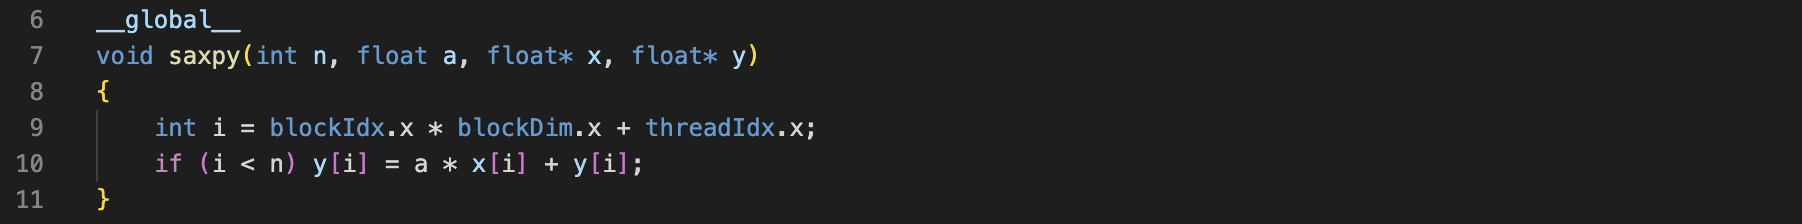
\includegraphics[width=\textwidth]{saxpy.png}
    \caption{Código de ejemplo \texttt{saxpy} que encontramos en \url{https://developer.nvidia.com/blog/how-implement-performance-metrics-cuda-cc/}
	Extraemos los recursos que utilizamos de esta página web.}
\end{figure}

\subsection{Ancho de banda de memoria.}

Para calcular el ancho de banda de memoria teórico utilizamos la fórmula

$$ BW_{Theorical} = T \cdot R $$

siendo $T$ el número de transferencias efectuadas por unidad de tiempo y $R$ la relación $\frac{bytes}{transferencia}$.

Mientras que para el cálculo del ancho de banda efectivo tenemos que

$$ BW_{Effective} = \frac{(R_{B} + W_{B})}{t} $$

donde $R_{B}$ es el número de bytes leídos por kernel y $W_{B}$ es el número de bytes
escritos por kernel.

\pagebreak

Nuestra gráfica utiliza memoria una memoria GDDR6, es decir, memoria de tipo \textit{double data rate},
y con una interfaz de memoria de 192 bits, funcionando a $1.75GHz$ en frecuencia base y $14GHz$ en la efectiva.

Para una \textit{RTX 2060} tenemos que

$$ BW_{Theorical} = 2 \cdot 14 \cdot 10^{9} \frac{transferencias}{segundo} \cdot 192 \frac{bits}{transferencia} \cdot \frac{1 \cdot byte}{ 8 \cdot bits} = 672 \frac{GB}{s} $$

si tomamos como la velocidad de la memoria la efectiva.

Por otra parte, tras ejecutar el programa, para la misma gráfica obtenemos un ancho de banda

$$ BW_{Effective} = 148.271504 \frac{GB}{s} $$

    \pagebreak
    \section{Cálculo del máximo de un vector.}

Aplicamos el conocimiento que encontramos en \url{https://developer.download.nvidia.com/assets/cuda/files/reduction.pdf}.

Nuestra estrategia al desarrollar el kernel es la siguiente.
A nivel de \textit{grid} vamos, por cada hebra, a ir buscando
el mayor número de entre los del índice $i$ y el siguiente
$i+blockDim\cdot gridDim$ mientras queden datos en el vector y una
vez hayamos hecho eso, sobre el máximo que encontremos para cada hebra,
reducir los máximos para cada hebra. Una vez terminamos este proceso,
volvemos a repetirlo para los máximos que hemos encontrado en el proceso
anterior.

Nuestro objetivo es el de encontrar el máximo por cada bloque y
después encontrar el máximo de entre todos estos bloques.

Como tamaño de \textit{grid} intentamos encontrar una relación entre tamaño del vector y
número de hebras utilizadas. Sin embargo, todas las pruebas nos dan peor que utlizar un tamaño
de bloque de 3072, por lo que establecemos ese el tamaño de bloque para utilizar por el kernel.

\begin{figure}[H]
    \centering
    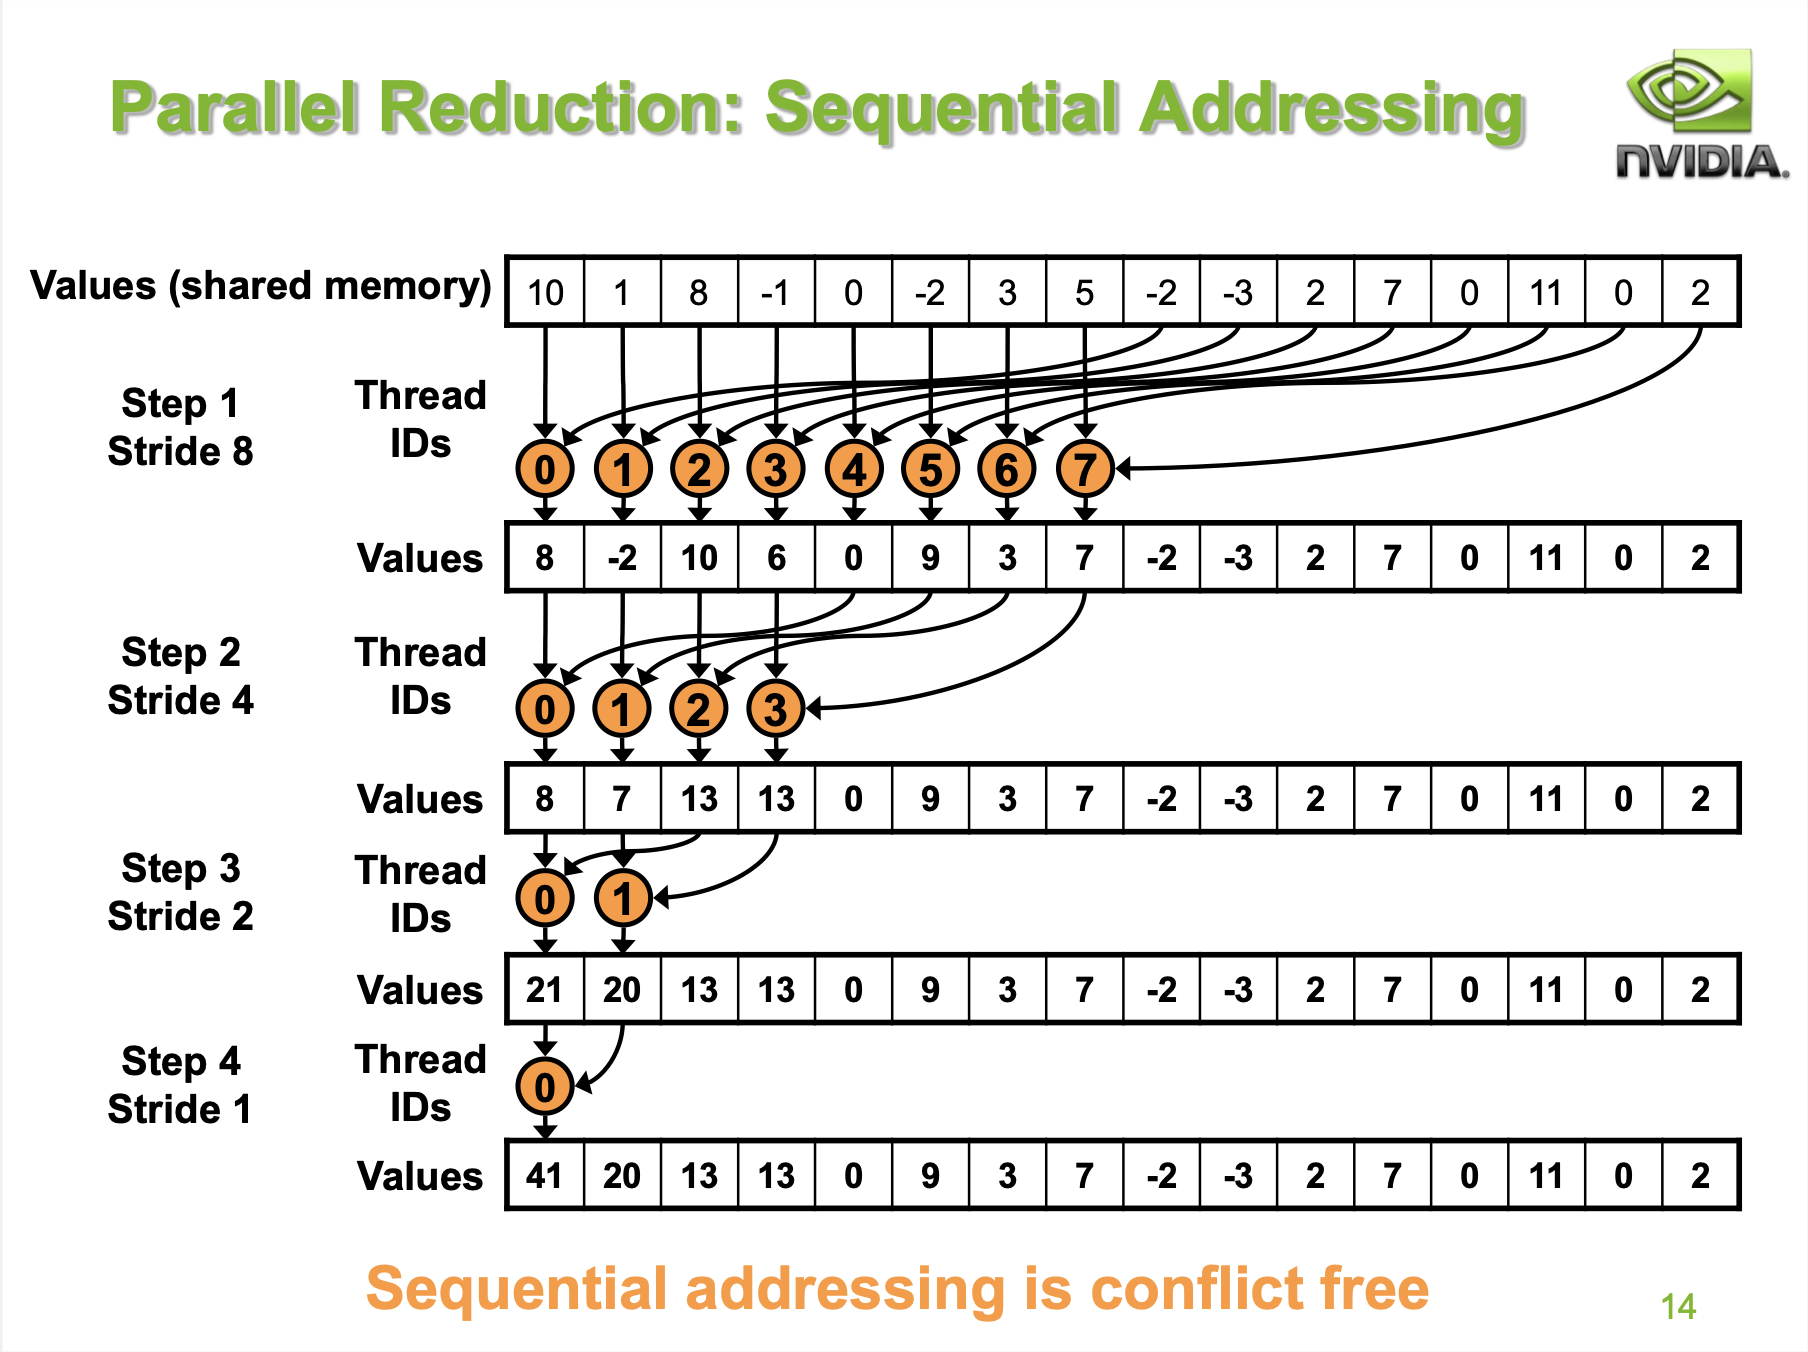
\includegraphics[width=8.5cm]{reduccion.png}
    \caption{Reducción paralela con direccionamiento secuencial para reducir un vector con la operación suma.
        Utilizamos esta misma estrategia en nuestro código.
        Extraído de \url{https://developer.download.nvidia.com/assets/cuda/files/reduction.pdf}.}
\end{figure}

\subsection{Análisis de la ejecución.}

Midiendo la utilización de los recursos de nuestra GPU descubrimos que la utilización del ancho de banda de memoria roza el
40\%, mientras que la capacidad de cómputo no llega al 60\%. Esto se debe a que aunque la ocupación de los \textit{Stream Processors}
alcanza su máximo efectivo aproximadamente el 90\% del tiempo los \textit{warps} están detenidos.
Analizando el código mediante la herramienta \textit{NVIDIA NSight Compute} descubrimos que la mayor parte del tiempo de ejecución
del kernel consiste en que el 30\% de los \textit{warps} acceden a memoria no residente en caché. El 55\% de las peticiones
de línea a caché de nivel uno fallaron y únicamente el 5\% de las peticiones de línea a caché de nivel dos tenían la línea preparada
para servirse.

Aun así, sin contar transferencias, nuestro algoritmo consigue aproximadamente una aceleración con respecto al algoritmo secuencial de CPU
de 68x. Si contamos transferencias encontramos con que este \textit{speedup} no alcanza el 2x.

Si el máximo número de entre todos los bloques lo encontramos en el \textit{host} con el algoritmo secuencial en vez de en el \textit{device}
obtenemos mejor aceleración.

Dado que la mayor parte del cuello de botella reside en las transferencias probamos a dividir los datos de entrada en distintos
bloques de forma que podamos, potencialmente, reducir la latencia. Para ello hacemos uso de \textit{streams}.
Descubrimos que, por alguna razón que no llegamos a investigar, la aceleración empeora hasta un 0.9x.

\subsection{Alternativas y trabajo futuro.}

Potencialmente nuestro \textit{kernel} podría mejorarse en gran medida cambiando el enfoque algorítmico y de transferencias de memoria.

Como alternativa podemos utilizar la librería \href{https://github.com/NVIDIA/thrust}{Thrust}, la cual junto a otras muchas utilidades
incluye un \textit{wrapper} para un algoritmo desarrollado por \textit{NVIDIA} para sus \textit{GPUs} para encontrar el máximo de un vector.

Si el código no fuese parte de otro algoritmo que se ejecutase en la GPU, sino que fuese un acelerador para la CPU, nos interesaría investigar
otras opciones como ciertas operaciones SIMD de la arquitectura x86 (o equivalentes según requiramos) como puede ser
\href{https://www.intel.com/content/www/us/en/docs/intrinsics-guide/index.html#text=_mm_cmplt_pd&ig_expand=1173}{\texttt{\_mm\_cmplt\_pd}.}

    \pagebreak
    \section{Multiplicación de matrices}

Se acabó lo que se daba. \textit{This is the end.}

Se nos pide escribir un \textit{kernel}\footnote{
No confundir con un \href{https://en.wikipedia.org/wiki/Kernel}{\textit{kernel}}.}\footnote{
Tampoco con \textit{Kernel}, el antiguo gato de la \href{https://etsiit.ugr.es}{ETSIIT}.}
que realize el producto de \href{http://matrices.net/tutorials.htm}{Matrices}.


Ilusionados, llenos de energía asi como de melancolía, comenzamos la resolución del ejercicio.

\subsection{Primera versión.}

Nos ponemos como objetivo acabar con un algoritmo correcto de forma que utilice
hebras y bloques independientemente de su eficiencia.

\begin{figure}[H]
    \centering
    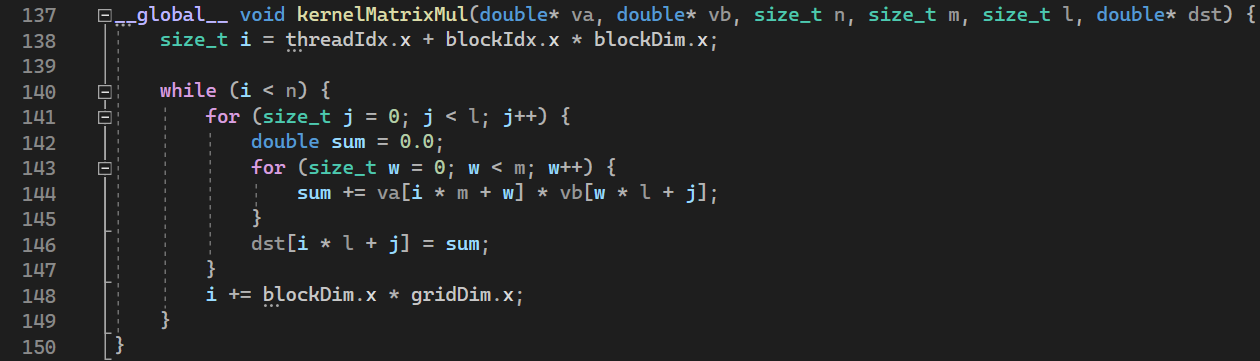
\includegraphics[width=\textwidth]{kernel1.png}
    \caption{Código de nuestro kernel para la primera versión. Únicamente considera que sea correcto.
    Cada hebra se encarga de una fila de la matriz que multiplica por la izquierda.}
\end{figure}

Conseguimos un factor de aceleración de x2 con respecto al algoritmo que ejecutamos en la CPU el cual no tiene consideraciones de optimización
adicionales. Para la medición tenemos en cuenta los tiempos de transferencia.

\begin{figure}[H]
    \centering
    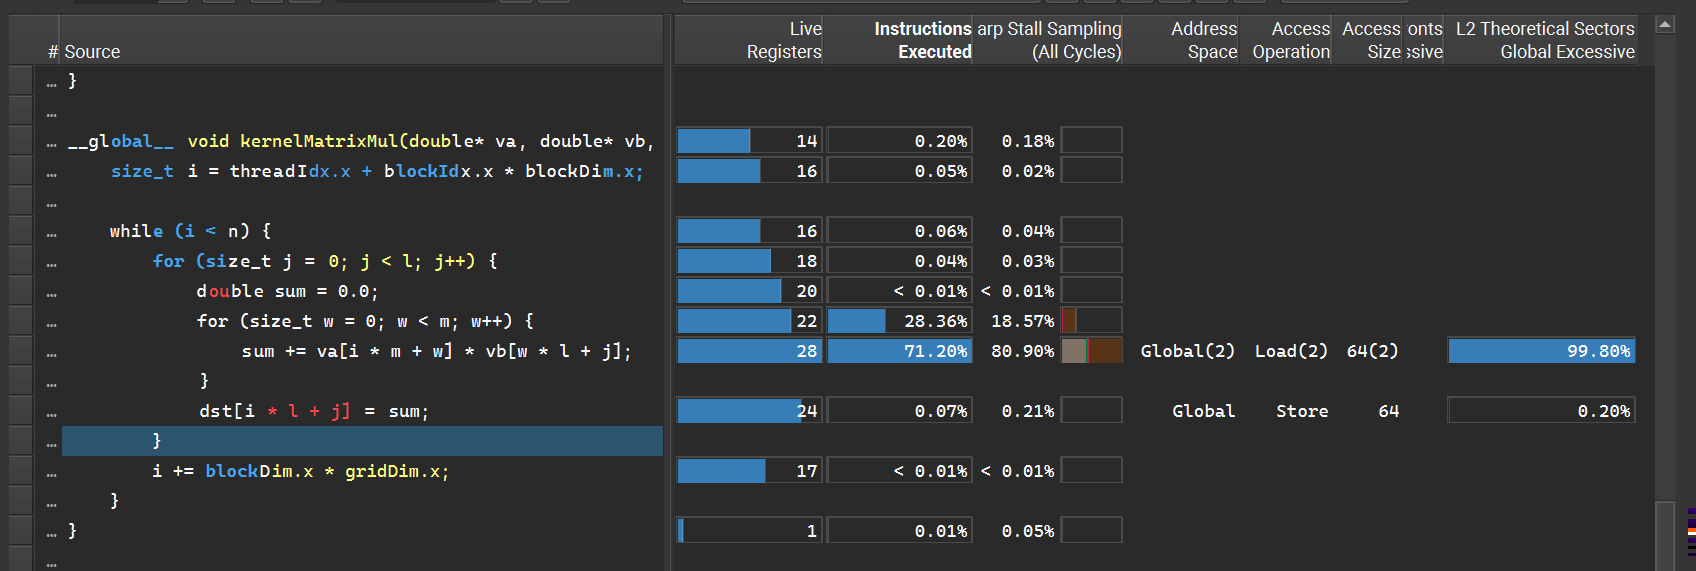
\includegraphics[width=\textwidth]{kernel1_bench.png}
    \caption{Analizador \textit{inline} de la herramienta \textit{NVIDIA NSight Compute}. Observamos cómo la mayor
    parte del esfuerzo computacional consiste tanto en acceder a memoria como en realizar la operacion de multiplicación y suma.}
\end{figure}

Tras analizar el algoritmo descubrimos que en nuestra GPU terminamos aproximadamente con un \textit{96\%} de fallos de caché de 
primer nivel y un \textit{22\%} de segundo.

\subsection{Segunda versión.}

Una vez terminada, probada y medida la primera versión iteramos sobre esta. Nuestro objetivo ahora será optimizar los
accesos a memoria.

La razón de elegir este como nuestro objetivo es que a nivel de \textit{warp}, si una hebra no puede recuperar memoria
todas las hebras de este, quedan a la espera. Es uno de los factores determinantes que dictan la ocupación de nuestra \textit{GPU}.

\begin{figure}[H]
    \centering
    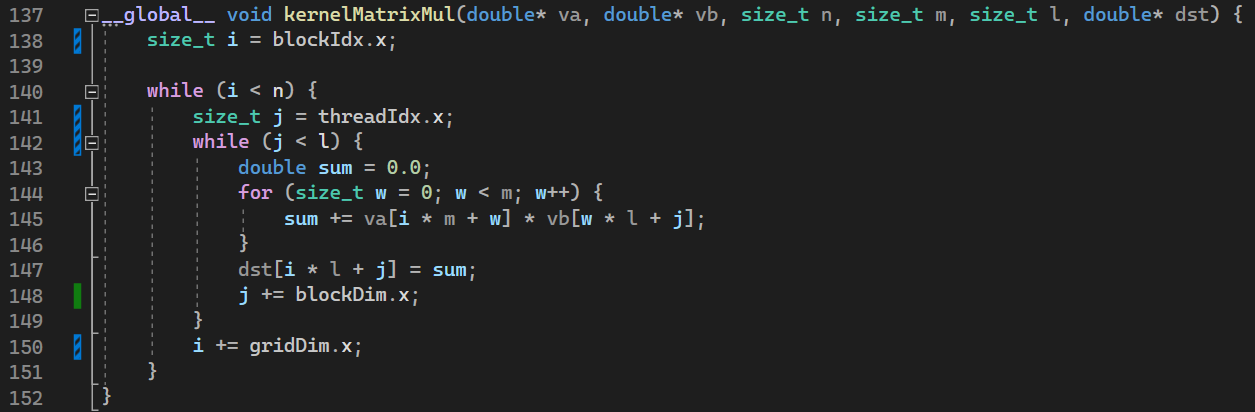
\includegraphics[width=\textwidth]{kernel2.png}
    \caption{Código de nuestro kernel para la segunda versión. Hacemos que cada bloque de hebras se encargue de una fila
    de la matriz que multiplica por la izquierda, favoreciendo la localidad especial, e intentando que ocurra de forma
    similar cuando se acceda a cada fila de la que multiplica por la derecha.}
\end{figure}

Conseguimos un factor de aceleración de x34\footnote{Con \href{https://www.youtube.com/watch?v=uC9d34cU2s8&t=73s}{risa maligna} incluida.} con respecto al algoritmo que ejecutamos en la CPU.
Para la medición tenemos en cuenta los tiempos de transferencia.

\begin{figure}[H]
    \centering
    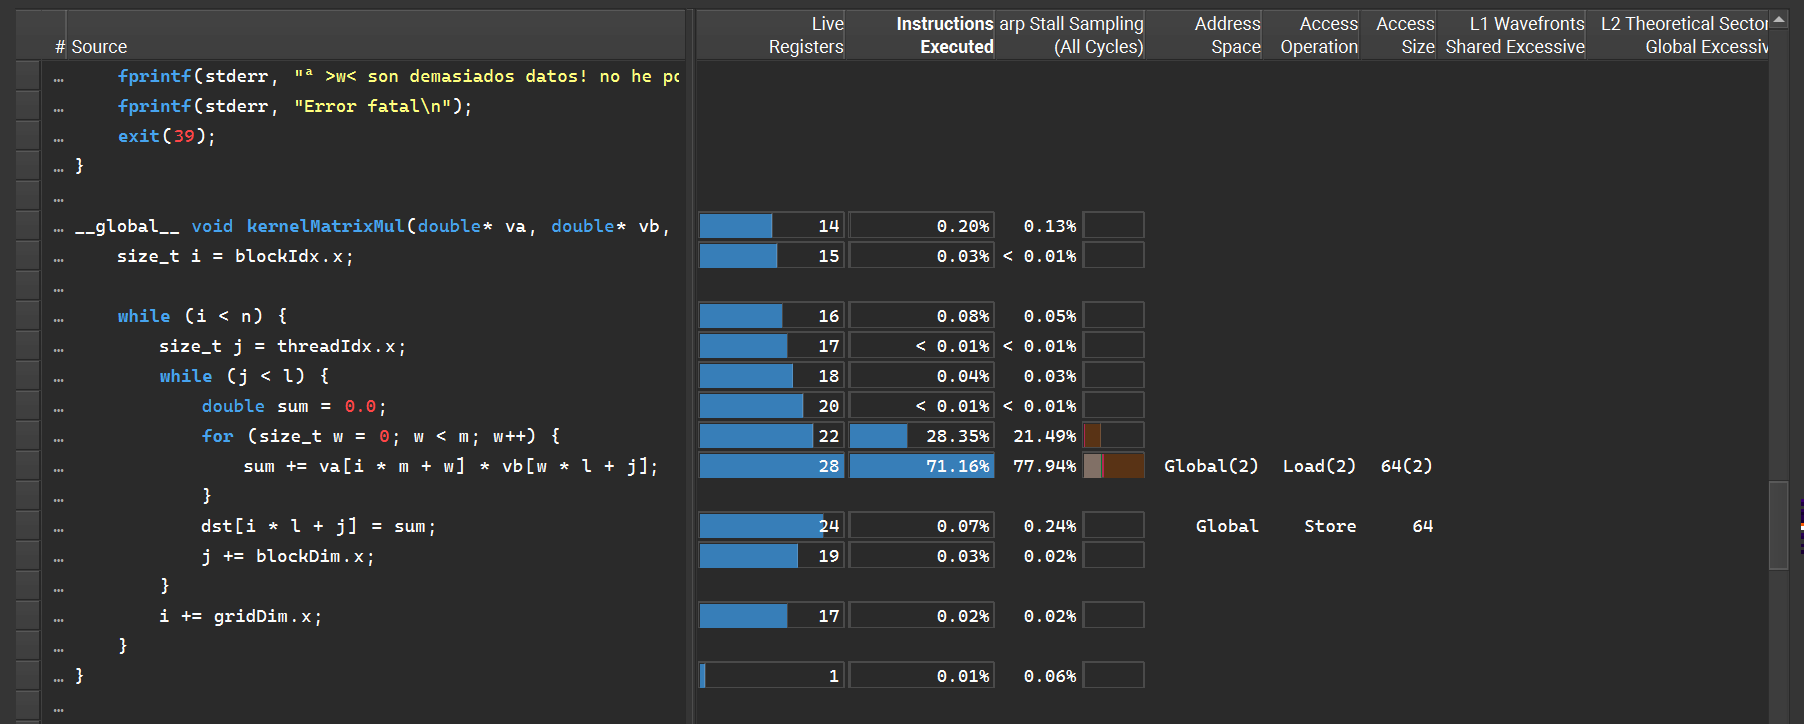
\includegraphics[width=\textwidth]{kernel2_bench.png}
    \caption{Analizador \textit{inline} de la herramienta \textit{NVIDIA NSight Compute}. Conseguimos que nuestra GPU tenga un \textit{94\%} de aciertos de caché al segundo
    nivel y un \textit{57.9\%} al primer nivel.}
\end{figure}

A lo mejor no tendremos segunda cita, pero lo cierto es que ya conoces lo penalizante que es realizar
accesos a memoria al \textit{tun-tún}.\footnote{Basado en un meme que ahora mismo no encuentro.}

\subsection{Alternativas y trabajo futuro.}

Si nuestro objetivo fuese seguir aprendiendo seguramente seguiríamos la entrada de blog que encontramos en \href{https://siboehm.com/articles/22/CUDA-MMM}{el siguiente enlace}.

Por otra parte, si quisiésemos acelerar la multiplicación de matrices en nuestro código utilizaríamos una librería como \href{https://docs.nvidia.com/cuda/cublas/}{cuBLAS}

Fin.


\end{document}
